%%%%%%%%%%%%%%%%%%%%%%%%%%%%%%%%%%%%%%%%%%%%%%%%%%%%%%%%%%%%%%%%%%%%%%%%%%%%%
% chapters/chapter-2.tex
%%%%%%%%%%%%%%%%%%%%%%%%%%%%%%%%%%%%%%%%%%%%%%%%%%%%%%%%%%%%%%%%%%%%%%%%%%%%%

\chapter{The Standard Model of Particle Physics}
\label{chap:theory}

The Standard Model (SM) of particle physics represents the most succesfull framework for describing the elementary constituents of our universe -all the known elementary particles and their interactions, with the notable exception of gravity. The SM is a relativistic quantum field theory (QFT), meaning that each particle is interpreted as an excitation of an underlying quantum field that permeates all space-time. The field content of the SM is limited to those with spin 0, 1/2, and 1. Spin-1/2 fields account for the fermion content, which include quarks and leptons and form the building blocks of matter; spin-1 fields describe the gauge bosons that mediate the strong and electroweak interactions; and a unique spin-0 field, the Higgs field, that is responsible for the mass generation via the Higgs mechanism. 

In the SM, quarks and leptons are distinguished by the types of interactions in which they participate -quarks engage in both strong and electroweak interactions while leptons only couples to the electroweak force- and also by a flavor quantum number, which results in six flavors of quarks and six flavors of leptons. Additionally, the SM fermions are divided into three generations, whith particles differing only in mass and flavor among such generations. Finally, the SM bosons are divided into three vector bosons, the mediators of the strong and electroweak interactions, and the scalar Higgs boson. A schematic overview of the particle content of the SM is provided in Figure~\ref{fig:smcontent}.

\begin{figure}[!htb]
\begin{center}
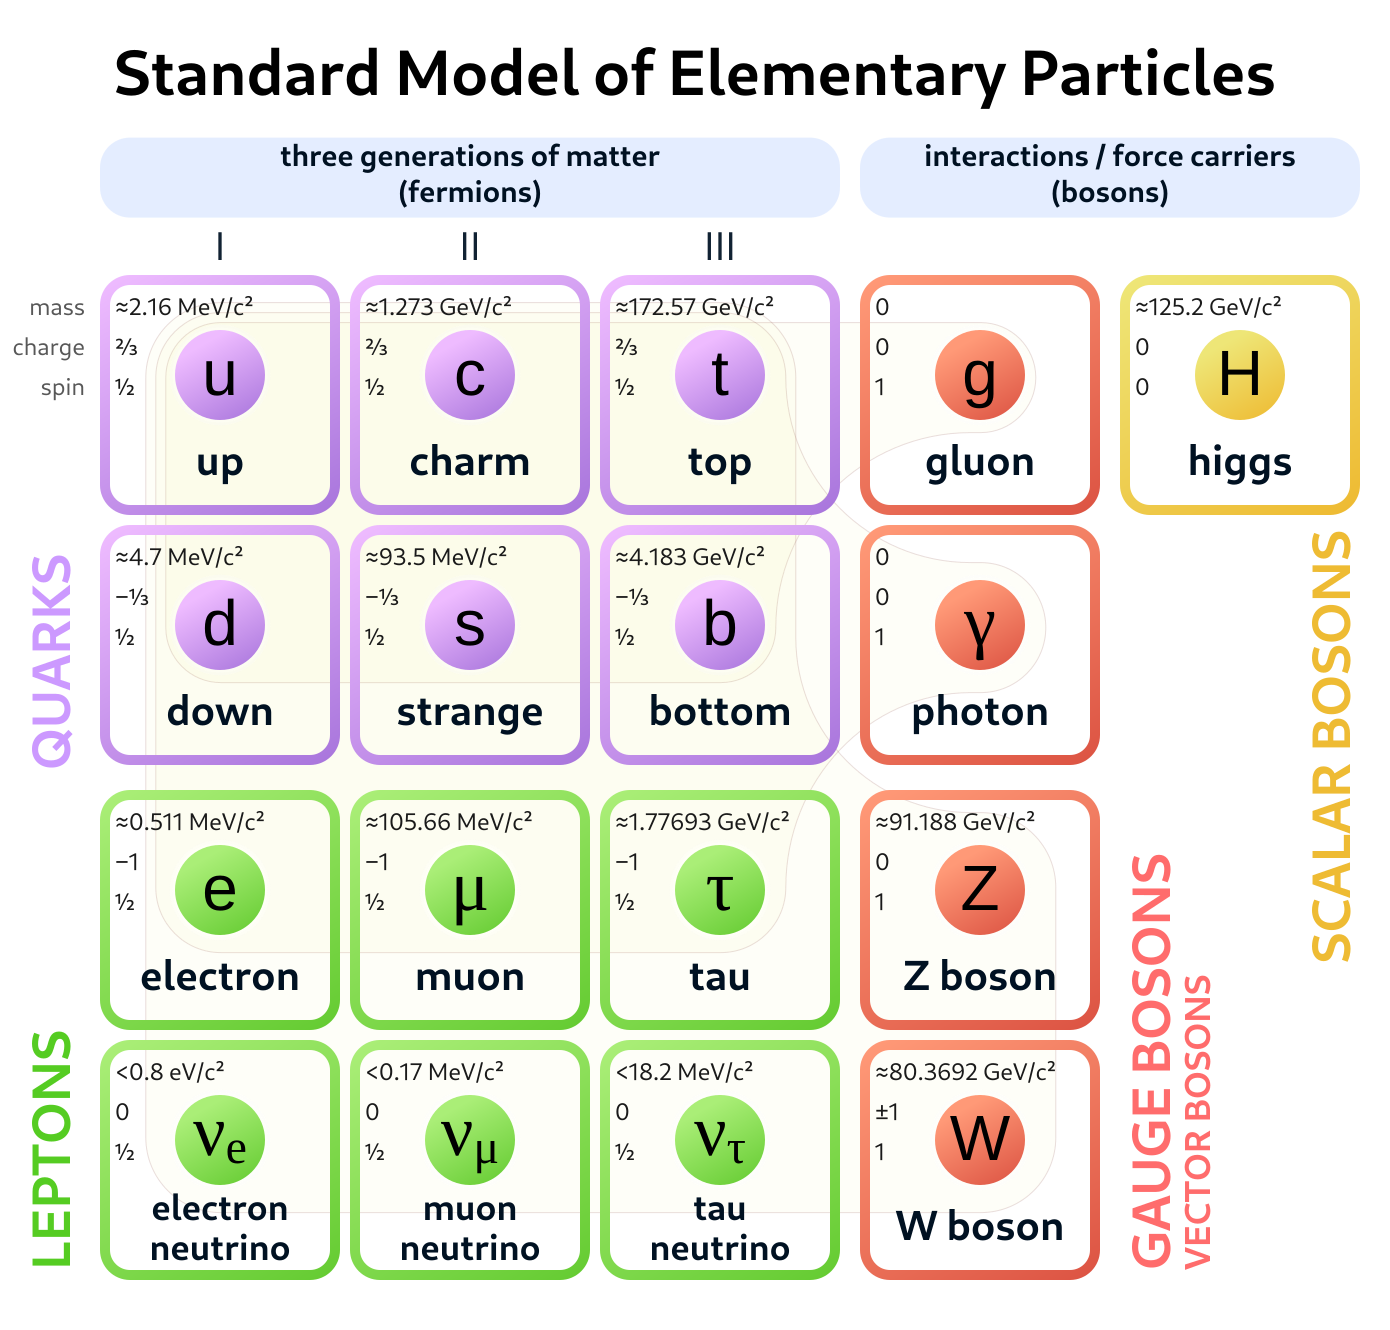
\includegraphics[width=0.8\textwidth]{figures/standard_model.png}\caption{Elementary particles of the Standard Model: 12 fundamental fermions and 5 fundamental bosons. Brown loops indicate which bosons (red) couple to which fermions (purple and green).}
\label{fig:smcontent}
\end{center}
\end{figure}

A compact and efficient mathematical formulation of the SM is achieved through the Lagrandian formalism. The dynamics and kinematics of the underlying fields are encoded in a Lagrangian density constructed to be invariant under both the global symmetries of special relativity (embodied in the Poincaré group) and local gauge transformations. The requirement for local gauge invariance leads to the symmetry group
\begin{equation}
\mathrm{SU}_C(3) \times \mathrm{SU}_L(2) \times \mathrm{U}_Y(1):
\label{SM_symmetry_group}
\end{equation}
$\mathrm{SU}_C(3)$ governs quantum chromodynamics (QCD), the theory of the strong interaction, acting on the gluon fields and all the particles that carry color charge; $\mathrm{SU}_L(2)$ is associated with the weak isospin and acts on the left-handed fermions as well as on the Higgs field; $\mathrm{U}_Y(1)$ corresponds to the weak hypercharge, and together with $\mathrm{SU}_L(2)$ forms the electroweak sector, giving rise to the electric charge after the electroweak symmetry breaking.

The SM provides a precise description of the particle content and their interactions, and has provided an extraordinary predictive power across a wide range of energies. Besides, despite its success, the SM is generally thought to be an effective theory as it leaves unanswered several fundamental questions, such as the incorporation of a quantum theory of gravity, the hierachy of mass scales, the origin of neutrino masses and the nature of dark matter, suggesting that the SM is not the ultimate theory of fundamental interactions. These limitations have motivated the search for extensions beyond the SM. Among these, supersymmetry (SUSY) has attracted significant attention. By postulating a symmetry between bosons and fermions, SUSY offers potential solutions to most of the SM's shortcomings, although experimental confirmation of supersymmetric partners have yet been observed.

This chapter provides an overview of the SM's main features, including its particle content and the construction of the Lagrangian, and discusses the shortcomings that motivate the exploration of extensions such as SUSY. Natural units, with $c=\hbar=1$, will be adopted throughout.
 
\section{Gauge Invariance in QFT}
\label{gauge_inv}

The principle of gauge invariance is cleanly illustrated by quantum electrodynamics (QED), the quantum field theory based on the $\mathrm{U}(1)$ symmetry group that describes electromagnetic interactions. Consider the Dirac fermionic field $\psi(x)$ with its adjoint defined as $\bar{\psi}(x)=\psi^\dagger(x)\gamma^0$. Under a local $\mathrm{U}(1)$ phase transformation, the field transforms as
\begin{equation}
\psi(x) \to \psi^\prime(x)=\mathrm{e}^{iq\chi(x)}\psi(x),
\end{equation}
where the phase $q\chi(x)$ may vary from point to point in space-time. If one applies this transformation to the free Dirac Lagrangian density
\begin{equation}
\mathcal{L}=\bar{\psi}(x)(i\gamma^\mu\partial_\mu-m)\psi(x),
\end{equation}
the Lagrangian transforms into
\begin{equation}
\mathcal{L}^\prime=\bar{\psi}^\prime(x)(i\gamma^\mu\partial_\mu-m)\psi^\prime(x).
\end{equation}
A straightforward calculation shows that
\begin{equation}
\mathcal{L}^\prime=\mathcal{L}-q\bar{\psi}(x)\gamma^\mu
(\partial_\mu\chi(x))\psi(x),
\end{equation}
revealing an extra term proportional to $\partial_\mu\chi(x)$, indicating that the free Dirac Lagrangian is not ivariant under local $\mathrm{U}(1)$ transformations. In order to restore local gauge invariance, the derivative $\partial_\mu$ must be replaced by the covariant derivative $D_\mu$, defined as
\begin{equation}
D_\mu=\partial_\mu+iqA_\mu(x),
\end{equation}
where $A_\mu(x)$ is a new gauge field. To have consistency under the local phase transformation, it is required that $A_\mu(x)$ transforms according to
\begin{equation}
A_\mu(x) \to A_\mu^\prime(x)=A_\mu - \partial_\mu\chi(x).
\end{equation}
The Dirac Lagrangian then beomes
\begin{equation}
\mathcal{L}=\bar{\psi}(x)(i\gamma^\mu D_\mu -m)\psi(x)=\bar{\psi}(x)(i\gamma^\mu -q\gamma^\mu A_\mu(x)-m)\psi(x).
\end{equation}
The new term $q\bar{\psi}(x)\gamma^\mu A_\mu(x)\psi(x)$ describes the interaction between the charged Dirac field and the electromagnetif field, i.e. identifying $A_\mu$ as the mediator of the electromagnetic interaction (the photon) and $q$ as the electric charge.

The full QED Lagrangian is obtained by adding the gauge-invariant kinetic term for the electromagnetic field:
\begin{equation}
\mathcal{L}=\bar{\psi}(x)(i\gamma^\mu D_\mu -m)\psi(x)-\frac{1}{4}F_{\mu\nu}(x)F^{\mu\nu}(x),
\end{equation}
where the field strenght tensor is defined as
\begin{equation}
F_{\mu\nu}(x)=\partial_\mu A_\nu(x)-\partial_\nu A_\mu(x).
\end{equation}
Thus, the requirement of local $\mathrm{U}(1)$ invariance implies the existence of a spin-1 gauge field $A_\mu(x)$, whose coupuling with the Dirac field not only ensures gauge invariance but also naturally represents the mediator of the electromagnetic interaction, the photon.

\section{Quantum Chromo Dynamics}
\label{sec:qcd}

Quantum chromodynamics (QCD) is the gauge theory of the color symmetry group $\mathrm{SU}_C(3)$ and describes the strong interaction between quarks and gluons. Quarks and gluons are the fundamental constituents of hadrons -composit particles (such as baryons and mesons) bound together by the strong force. Only particles carrying non-zero color charge interact strongly; therefore, colorless leptons do not feel the strong interaction.

There are three color charges, conventionally labeled $r$, $g$, and $b$, corresponding to three orthogonal states in the $\mathrm{SU}(3)$ color space. Each quark flavor forms a triplet in the fundamental representation of $\mathrm{SU}(3)$, while antiquarks belong to the conjugate representation, carrying the anticolors $\bar{r}$, $\bar{g}$, and $\bar{b}$. The strong interaction is mediated by eight massless gluons associated with the eight generators of $\mathrm{SU}(3)$, an exact symmetry that ensures invariance under unitary transformations in color space.

The QCD Lagrangian density is given by:
\begin{equation}
\mathcal{L}_{QCD}=\sum_q \bar{\psi}_{q,a} (i\gamma_\mu D^\mu_{ab} -m_q \delta_{ab})\psi_{q,b}-\frac{1}{4}F_{\mu\nu}^A F^{\mu\nu}_A,
\end{equation}
where the sum runs over quark flavors $q$. Here, $\gamma^\mu$ are the Dirac matrices, $\psi_{q,a}$ is the quark field of flavor $q$ and mass $m_q$, with the color index $a=1,2,3$, and $\bar{\psi_{q,a}}$ its Dirac adjoint.

The gauge covariant derivative $D^\mu_{ab}$ is defined as:
\begin{equation}
D^\mu_{ab}=\delta_{ab}\partial^\mu + ig_S (t^A)_{ab}G^\mu_A,
\end{equation}
where $g_S$ is the strong coupling constant, $G^\mu_A$ (with $A=1,...,8$) are the gluon fields, and the matrices $t^A_{ab}=\lambda^A_{ab}/2$ are the generators of $\mathrm{SU}(3)$, with $\lambda^A$ the Gell-Mann matrices. These generators satisfy the commutation relation:
\begin{equation}
[t_A,t_B]=if_{ABC}t_C,
\end{equation}
with $f_{ABC}$ being the totally anstisymmetric structure constants of $\mathrm{SU}(3)$.

The gluon field strength tensor is given by:
\begin{equation}
F_{\mu\nu}^A=\partial_\mu G_\nu^A - \partial_\nu G_\mu^A - g_S f_{ABC} G_\mu^B G_\nu^C.
\end{equation}

Color charge conservation requires that gluons themselves carry color. Since quarks carry one of the three colors and antiquarks one of the three anticolors, each gluon must carry both a color and an anticolor. Although there are nine possible color-anticolor independend combinations, only eight correspond to the independent physical gluon states, forming an octet. One way these states can be represented is the following:
\begin{equation}
r\bar{g}, \quad g\bar{r}, \quad r\bar{b}, \quad b\bar{r}, \quad g\bar{b}, \quad b\bar{g}, \quad \frac{1}{\sqrt{2}}(r\bar{r}-g\bar{g}), \quad \frac{1}{\sqrt{6}}(r\bar{r}+g\bar{g}-2b\bar{b}).
\end{equation}
In addition, there exist another independent combination,
\begin{equation}
\frac{1}{\sqrt{3}}(r\bar{r}+b\bar{b}+g\bar{g}),
\end{equation}
which is inveriant under $\mathrm{SU}(3)$ rotations. However, $\mathrm{SU}(3)$ is defined as the group of $3\times 3$ unitary matrices with determinant one, which restricts its generators to be traceless -yielding only eight independent generators (the Gell-Mann matrices). Including a ninth generator would extend the symmetry to $\mathrm{U}(3)$, and the additional generator would correspond to a color singlet state. Since QCD is based on $\mathrm{SU}(3)$, only the eight color-octet gluons are physical. Moreover, the absence of a physical color-neutral gluon is constistent with the observation that hadrons, which are color singlets, do not experience long-range interactions.

Ultimately, QCD not only provides a detailed description of quark and gluon dynamics but also explains why only color-neutral states are observed in nature. 


\subsection{Color Confinment, Asymptotic freedom, Hadronization and Jets}
\label{subsec:confinment}


Quarks and gluons are the fundamental fields of QCD, yet free quarks and gluons have never been observed. This is due to color confinment, which requires that only color-neutral (singlet) states can exist as free particles. In practice, quarks are always bound into hadrons, composite particles such as baryons (typically three-quark states like proton and neutrons) and mesons (quark-antiquark pairs). Color singlet states made up of gluons only (``glueballs'') are also consistent with color confinment, but have so far not been experimentally observed.

There is currently no analytical proof of color confinement, though a qualitative picture can be obtained by considering two quarks being pulled apart. As they separate, the quarks interact by exchanging virtual gluons, which themselves carry color. This leads to gluon self-interactions and the formation of a narrow flux tube with constant energy density between the quarks. Consequently, the energy stored in the gluon field increases linearly with distance, making it energetically impossible to isolate individual quarks. Instead, when the energy in the flux tube becomes sufficiently high, it is more favorable to create a new quark-antiquark pair, a process knows as hadronization. In high-energy experiments, this mechanism results in the formation of narrow hadronic jets that reflect the original quark directions.

In contrast to the strong coupling at low energies responsible for confinement, QCD exhibits asymptotic freedom: the strong interaction becomes weaker at higher energy scales, allowing perturbative calculations. This behavior originates from vacuum polarization effects in QCD. Virtual quark-antiquark pairs tend to screen a physical color charge, while virtual gluon pairs, carrying both color and anticolor, produce an anti-screening effect. For QCD, with three colors ($N_C=3$) and six quark flavors ($N_f=6$), anti-screening dominates, so that the effective coupling $\alpha_S$ decreases with increasing momentum transfer $Q^2$. In perturbative QCD the running coupliong is expressed as
\begin{equation}
\alpha_S(Q^2)=\frac{\alpha_S(Q^2)}{1+\beta_0\alpha_S(\mu^2)\mathrm{ln}\left( \frac{Q^2}{\mu^2}\right)},
\end{equation}
with
\begin{equation}
\beta_0=\frac{11N_C -2N_f}{12\pi}.
\end{equation}
At high energies, quarks behave as quasi-free particles, while at low energies $\alpha_S$ grows until it diverges at the scale $\Lambda_{QCD} \sim 332 \pm 17$ MeV, marking the onset of confinement.

Thus, QCD displayis a dual nature: asymptotic freedom at high energy permits a perturbative treatment of quark gluon interactions, whereas at low energies, color confinement ensures that only color-neutral hadrons are observed.

\section{Electroweak Theory}
\label{ew_theory}

The electroweak theory unifies the electromagnetic and weak interactions under the gauge group
\begin{equation}
\mathrm{SU}_L(2) \times \mathrm{U}_Y(1)
\end{equation}
with the gauge fields $W_\mu^1$, $W_\mu^2$, and $W_\mu^3$ associated with $\mathrm{SU}(2)$ (carrying weak isospin) and $B_\mu$ associated with $\mathrm{U}(1)$ (carrying hypercharge). Its Lagrandian density is given by:
\begin{equation}
\mathcal{L}_{EW}=-\frac{1}{4}\sum_{A=1}^3 F_{\mu\nu}^A F_A^{\mu\nu}-\frac{1}{4}B_{\mu\nu}B^{\mu\nu}+\sum_j \left[ \bar{\psi}_L^j i \gamma^\mu D_\mu \psi_L^j + \bar{\psi}_R^j i \gamma^\mu D_\mu \psi_R^j \right],
\end{equation}
where the index $j$ runs over the three fermion generations. The $\mathrm{SU}(2)$ field strength tensor is
\begin{equation}
F_{\mu\nu}^A=\partial_\mu W^A_\nu-\partial_\nu W_\mu^A-g_W \epsilon_{ABC} W_\mu^B W_\nu^C,
\end{equation}
and the $\mathrm{U}(1)$ tensor is
\begin{equation}
B_{\mu\nu}=\partial_\mu B_\nu - \partial_\nu B_\mu.
\end{equation}
Here, $g_W$ is the $\mathrm{SU}(2)$ coupling constant and $\epsilon_{ABC}$ is the totally antisymmetric Levi-Civita symbol.

The fermion fields are split into left- and right-handed components. For a Dirac field $\psi$, chirality is defined by
\begin{equation}
\gamma_5= i \gamma^0\gamma^1\gamma^2\gamma^3,
\end{equation}
with eigenvalues $-1$ for left-handed (LH) and $+1$ for right-handed (RH) states. The projections are given by
\begin{equation}
\psi_L=\frac{1-\gamma_5}{2}\psi, \quad \psi_R=\frac{1+\gamma_5}{2}\psi,
\end{equation}
and similarly for the adjoints. Since only the LH particles (and RH antiparticles) participate in charged weak interactions, LH fields are arranged in $\mathrm{SU}(2)$ doublets, while RH fields are $\mathrm{SU}(2)$ singlets.

The covariant derivative is defined as
\begin{equation}
D_\mu = \partial_\mu + ig_W \sum_{A=1}^3 T^A W_\mu^A+ ig^\prime \frac{Y}{2}B_\mu,
\end{equation}
where $T^A$ are the $\mathrm{SU}(2)$ generators satisfying
\begin{equation}
[T^A,T^B]=i\epsilon_{ABC}T^C,
\end{equation}
and $Y$ is the weak hypercharge. The electric charge $Q$ is given by the Gell-Mann-Nishijima relation,
\begin{equation}
Q=T^3+\frac{1}{2}Y.
\end{equation}
For the three fermion families, the LH weak isospin doublets are
\begin{equation}
\binom{\nu_\ell}{\ell^-}_L \quad \mathrm{and} \quad \binom{q_u}{q_d^\prime}_L,
\end{equation}
while the RH singlets are $l_R^-$, $q_{uR}$, and $q_{dR}^\prime$. Here, $q_d^\prime$ denotes the weak eigenstates, which are mixtures of the mass eigenstates $q_d$ via the Cabibbo-Kobayashi-Maskawa matrix.

Charged current (CC) interactions arise from the fields $W_\mu^1$ and $W_\mu^2$, which combine to form the charged bosons:
\begin{equation}
W_\mu^\pm = \frac{1}{\sqrt{2}}(W_\mu^1 \mp i W_\mu^2),
\end{equation}
with the corresponding ladder operators $T^\pm = T^1 \mp iT^2$. The CC Lagrangian is
\begin{equation}
\mathcal{L}_{CC}= \frac{g_W}{2\sqrt{2}} \sum_j \left[ \bar{\psi}_L^j \gamma^\mu (1-\gamma_5)(T^+W_\mu^+ + T^- W_\mu^-)\psi_L^j\right],
\end{equation}
which exhibits a pure V-A structure (i.e. ``pure vector minus axial-vector''), coupling only to LH fermions and RH antifermions.

Neutral currents (NC) involve the neutral bosons, which arise as orthogonal combinations of $W_\mu^3$ and $B_\mu$:
\begin{equation}
\begin{cases}
      A_\mu = \cos \theta_W B_\mu + \sin \theta_W W_\mu^3 \\
      Z_\mu = -\sin \theta_W B_\mu + \cos \theta_W W_\mu^3
    \end{cases},
\end{equation}
with the weak mixing angle $\theta_W$. $Z_\mu$ is identified with the mediator of the weak NC and $A_\mu$ with the photon. The photon couples universally with strength $e$, where
\begin{equation}
e=g_W\sin \theta_W=g^\prime \cos \theta_W \implies \frac{g^\prime}{g_W}= \tan \theta_W.
\end{equation}
The NC Lagrangian is given by
\begin{equation}
\mathcal{L}_{NC}= \frac{g_W}{2 \cos \theta_W} \sum_j \bar{\psi}^j \gamma^\mu \left( g_V^j - g_A^j \gamma_5\right) \psi^j Z_\mu,
\end{equation}
with vector and axial couplings defined as
\begin{equation}
g_V^j = T^{3j}-2Q^j \sin^2\theta_W, \quad g_A^j = T^{3j}.
\end{equation}
Alternatively, defining
\begin{equation}
g_L^j = \frac{1}{2}(g_V^j+g_A^j) \quad \mathrm{and} \quad g_R^j=\frac{1}{2}(g_V^j-g_A^j),
\end{equation}
the NC interaction can be written as
\begin{equation}
\mathcal{L}_{NC}=\frac{g_W}{2 \cos \theta_W} \sum_j \bar{\psi}^j \gamma^\mu \left[ g_L^j (1-\gamma_5) + g_R^j(1+\gamma_5)\right] \psi^j Z_\mu,
\end{equation}
demonstrating that, unlike the charged currents, both LH and RH components participate in neutral interactions.

In summary, the electroweak theory, with its chiral structure and well-defined gauge interactions, successfully unifies electromagnetic and weak forces while predicting the observed phenomena of charged and neutral current interactions.


\section{Higgs Sector}


The electroweak model described in Section \ref{ew_theory} unifies electromagnetic and weak interactions by introducing gauge bosons as force mediators through the requirement of gauge invariance. This invariance ins mantained by replacing the partial derivative $\partial_\mu$ with the covariant derivative $D_\mu$, which introduces new vector fields. However, in gauge theories it is not permissible to include explicit mass terms for these gauge bosons, as such terms would break local gauge invariance. For example, in QED (discussed in Section \ref{gauge_inv}), a poton mass term
\begin{equation}
\frac{1}{2}m_\gamma^2 A_\mu A^\mu
\end{equation}
would transform under
\begin{equation}
A_\mu \to A_\mu^\prime = A_\mu - \partial_\mu \chi
\end{equation}
to
\begin{equation}
\frac{1}{2} m_\gamma^2 (A_\mu - \partial_\mu \chi)(A^\mu - \partial^\mu \chi),
\end{equation}
which clearly does not equal the original mass term. Thus, the $\mathrm{U}(1)$ gauge symmetry of QED, as well as the $\mathrm{SU}(3)$ of QCD and the $\mathrm{SU}(2)$ of weak isospin, requires massless gauge bosons. This is acceptable for photons and gluons, but poses a problem for the electroweak theory where the $W^\pm$ and $Z$ bosons are experimentally known to be massive.

Similarly, explicit fermion mass terms of the form
\begin{equation}
-m_f (\bar{\psi}_R\psi_L + \bar{\psi}_L \psi_R)
\end{equation}
are not allowed, because the left-handed fermions transform as $\mathrm{SU}(2)$ doublets while the right-handed ones are singlets, making such mass terms non-invariant under $\mathrm{SU}(2)\times \mathrm{U}(1)$.

The solution to this problem is provided by spontaneous symmetry breaking via the Higgs mechanism. In this framework, the $\mathrm{SU}(2)\times \mathrm{U}(1)$ symmetry remains intact in the Lagrangian, but the vacuum state does not respect the symmetry. Interactions with the scalar Higgs field then generate masses for the $W^\pm$ and $Z$ bosons, as well as for the fermions, without explicitly breaking the gauge invariance of the theory. This mechanism, introduced by Higgs, Brout, Englert and others in the 1960s, is the cornerstone of the SM.


\subsection{Spontaneous Symmetry Breaking}

Consider a complex scalar field
\begin{equation}
\phi = \frac{1}{\sqrt{2}}(\phi_1+i\phi_2)
\end{equation}
with potential
\begin{equation}
V(\phi) = \mu^2 \phi^* \phi + \lambda (\phi^*\phi)^2.
\end{equation}
Its Lagrangian density is
\begin{equation}
\mathcal{L}=(\partial_\mu \phi)^*(\partial^\mu \phi) - V(\phi).
\end{equation}
Expressed in terms of the real fields $\phi_1$ and $\phi_2$, it becomes
\begin{equation}
\mathcal{L}=\frac{1}{2}(\partial_\mu\phi_1)^2 + \frac{1}{2}(\partial_\mu \phi_2)^2 - \frac{1}{2}\mu^2 (\phi_1^2+\phi^2_2) - \frac{1}{4}\lambda (\phi_1^2+\phi_2^2)^2.
\end{equation}
This Lagrangian is invariant under global $\mathrm{U}(1)$ transformations, $\phi\to\mathrm{e}^{i\alpha}\phi$, since $\phi^*\phi$ is unchanged.

For $\lambda>0$ the potential is bounded from below, and its minimum depends on the sign of $\mu^2$:
\begin{itemize}
\item[-] if $\mu^2>0$, the minimum is at $\phi_1=\phi_2=0$,
\item[-] if $\mu^2<0$, the minimum is not unique but lies on a circle defined by
\begin{equation}
\phi_1^2+\phi_2^2=\frac{-\mu^2}{\lambda} = v^2,
\end{equation}
\end{itemize}
with $v$ the vacuum expectation value (VEV). Choosing a specific vacuum state (say, $\phi_1=v$ and $\phi_2=0$) spontaneously breaks the global $U(1)$ symmetry.

Expanding around the chosen vacuum,
\begin{equation}
\phi_1(x)=v+\eta(x), \quad \phi_2(x)=\xi(x),
\end{equation}
so that
\begin{equation}
\phi(x)=\frac{1}{\sqrt{2}} \left( v + \eta(x) + i \xi(x)\right),
\end{equation}
the Lagrangian becomes
\begin{equation}
\mathcal{L}=\frac{1}{2}(\partial_\mu\eta)^2 + \frac{1}{2}(\partial_\mu\xi)^2 - \frac{1}{2}(2\lambda v^2)\eta^2 -V_{int}(\eta,\xi),
\end{equation}
where the quadratic term in $\eta$ gives it a mass $m_\eta=\sqrt{2\lambda v^2}$ while $\xi$ remains massless. The massless scalar $\xi$ is the Goldstone boson, arising from the broken continuous symmetry.

This spontaneous symmetry breaking mechanism can be embedded in a local $\mathrm{U}(1)$ gauge theory. In that case, one replaces the ordinary derivative with the covariant derivative
\begin{equation}
D_\mu = \partial_\mu + igB_\mu,
\end{equation}
where $B_\mu$ is a massless gauge field that transforms as
\begin{equation}
B_\mu \to B_\mu^\prime= B_\mu - \partial_\mu \alpha(x),
\end{equation}
and the Lagrangian becomes
\begin{equation}
\mathcal{L}=-\frac{1}{4}F_{\mu\nu}F^{\mu\nu}+(D_\mu\phi)^*(D^\mu\phi) - \mu^2\phi^*\phi - \lambda(\phi^*\phi)^2,
\end{equation}
with $F_{\mu\nu}=\partial_\mu B_\nu - \partial_\nu B_\mu$.

For $\mu^2<0$ the field acquires a VEV, and writing
\begin{equation}
\phi(x) = \frac{1}{\sqrt{2}} \left( v + \eta(x9 +i\xi(x)\right),
\end{equation}
one finds, besides the kinetic and potential terms for $\eta$ and $\xi$, a gauge-dependent mixing term $gvB_\mu\partial^\mu\xi$ and a mass term for the gauge field, $\frac{1}{2}g^2v^2B_\mu B^\mu$. By choosing the unitary gauge, where one performs a gauge transformation to set $\xi(x)=0$, the Lagrangian simplifies to
\begin{equation}
\mathcal{L}=\frac{1}{2}(\partial_\mu\eta)^2 - \lambda v^2\mu^2 - \frac{1}{4}F_{\mu\nu}F^{\mu\nu}+\frac{1}{2}g^2v^2B_\mu B^\mu + \mathrm{interaction terms}.
\end{equation}
Thus, the spetrum consists of a massive scalar field $\eta$ with $m_\eta=\sqrt{2\lambda v^2}$ (the Higgs boson) and a massive gauge boson $B_\mu$ with mass $m_B=gv$. The original Goldstone boson $\eta$ has been ``eaten'' by the gauge field, becoming its longitudilal polarization. This is the essence of the Higgs mechanism.


\subsection{The Higgs Mechanism in the Standard Model}

The Higgs mechanism is incorporated into the SM to spontaneously break the $SU_L(2) \times U_Y(1)$ electroweak symmetry down to the electromagnetic $U_\mathrm{em}(1)$ symmetry, generating masses for the $W^\pm$ and $Z$ bosons while keeping the photon massless.

To preserve the fundamental $SU_L(2) \times U_Y(1)$ gauge symmetry, the simplest approach introduces a complex scalar $SU_L(2)$ doublet with hypercharge $Y = +1$:
\begin{equation}
\phi = \begin{pmatrix} \phi^+ \\ \phi^0 \end{pmatrix} = \frac{1}{\sqrt{2}} \begin{pmatrix} \phi_1 + i\phi_2 \\ \phi_3 + i\phi_4 \end{pmatrix},
\end{equation}
where $\phi^+$ carries electric charge $+1$ and $\phi^0$ is neutral.

The Higgs potential is given by
\begin{equation}
V(\phi) = \mu^2 \phi^\dagger \phi + \lambda(\phi^\dagger \phi)^2,
\end{equation}
which for $\lambda > 0$ and $\mu^2 < 0$ has degenerate minima satisfying
\begin{equation}
\phi^\dagger \phi = -\frac{\mu^2}{2\lambda} = \frac{v^2}{2},
\end{equation}
where $v$ is the vacuum expectation value (VEV).

To break $SU_L(2) \times U_Y(1)$ while preserving $U_{em}(1)$, only the neutral component can acquire a non-zero VEV. Choosing the vacuum state and expanding in the unitary gauge:
\begin{equation}
\phi(x) = \frac{1}{\sqrt{2}} \begin{pmatrix} 0 \\ v + h(x) \end{pmatrix},
\end{equation}
where $h(x)$ is the physical Higgs field. In this way, the symmetry is broken such that the electromagnetic generator $Q = T^3+\frac{Y}{2}$ remains unbroken.

The gauge boson masses are generated by the kinetic term $(D_\mu\phi)^\dagger(D^\mu\phi)$ in the Lagrangian, where the covariant derivative is given by
\begin{equation}
D_\mu = \partial_\mu + ig_W \sum_{A=1}^3 T^A W_\mu^A + ig^\prime \frac{Y}{2}B_\mu.
\end{equation}
Expanding this term yields mass terms for the gauge bosons:
\begin{equation}
\mathcal{L}_{\text{mass}} = \frac{1}{8}v^2 \left[ 2g_W^2(W^{+\mu}W^-_\mu) + (W^{3\mu}, B^\mu) \begin{pmatrix} g_W^2 & -g_Wg' \\ -g_Wg' & g'^2 \end{pmatrix} \begin{pmatrix} W^3_\mu \\ B_\mu \end{pmatrix} \right].
\end{equation}

In particular, the charged $W^\pm$ fields, defined as
\begin{equation}
W^\pm_\mu = \frac{1}{\sqrt{2}}(W_\mu^1 \mp iW_\mu^2),
\end{equation}
acquire masses $m_W=\frac{1}{2}vg_W$.
The neutral fields $W_\mu^3$ and $B_\mu$ mix; diagonalization yields the massless photon
\begin{equation}
A_\mu = \frac{g^\prime W_\mu^3 + g_W B_\mu}{\sqrt{g_W^2+g^{\prime 2}}},
\end{equation}
and the $Z$ boson
\begin{equation}
Z_\mu = \frac{g_W W_\mu^3 - g^\prime B_\mu}{\sqrt{g_W^2+g^{\prime 2}}},
\end{equation}
with mass $m_Z = \frac{1}{2}v\sqrt{g_W^2+g^{\prime 2}}$.

The Higgs boson mass, $m_h = \sqrt{2\lambda}v$, is determined by the quadratic term in the scalar potential.

Fermion masses arise through Yukawa interactions with the Higgs doublet. Since only $\phi^0$ acquires a VEV, generating masses for up-type quarks requires the charge-conjugate doublet:
\begin{equation}
\tilde{\phi} = i\sigma_2 \phi^* = \begin{pmatrix} \phi^{0*} \\ -\phi^- \end{pmatrix}.
\end{equation}

The Yukawa Lagrangian is
\begin{equation}
\mathcal{L}_{\text{Yukawa}} = -\sum_{i,j} \left[ Y^e_{ij} \bar{L}_i \phi e_{R,j} + Y^d_{ij} \bar{Q}_i \phi d_{R,j} + Y^u_{ij} \bar{Q}_i \tilde{\phi} u_{R,j} \right] + \text{h.c.},
\end{equation}
where $L_i$ and $Q_i$ denote the lepton and quark $SU_L(2)$ doublets of generation $i$, and $Y^{e,d,u}$ are the Yukawa coupling matrices. After symmetry breaking, fermion masses are
\begin{equation}
m_f = \frac{Y_f v}{\sqrt{2}}.
\end{equation}

Therefore, the Higgs mechanism provides a unified framework for mass generation in the SM: the $W^\pm$ and $Z$ bosons acquire mass through their coupling to the Higgs VEV, fermions obtain mass via Yukawa couplings, and the photon remains massless as required by the unbroken $U_\mathrm{em}(1)$ symmetry.


\section{Shortcomings of the Standard Model}

The SM, while being the most successful theory to date for describing fundamental particles and their interactions up to the TeV scale, is nonetheless believed to be an effective field theory that must be embedded in a more fundamental framework. Several theoretical and experimental observations point to physics beyond the Standard Model (BSM).

\textbf{Gravity.} The SM does not incorporate general relativity. At the Planck scale ($M_P \sim 10^{19}$ GeV), quantum gravitational effects become important, yet no consistent quantum theory of gravity exists within the SM. The gravitational interaction is fundamentally different from the gauge interactions, and attempts to quantize gravity using standard QFT methods lead to a non-renormalizable theory.


\textbf{Hierarchy problem.} The Higgs mass receives quadratic corrections from quantum loops:
\begin{equation}
\delta m_h^2 \sim \frac{\Lambda^2}{16\pi^2} \left( 6\lambda + \frac{3}{2}(g^2 + g'^2) - 12y_t^2 \right),
\end{equation}
where $\Lambda$ is the cutoff scale and $y_t$ is the top Yukawa coupling. If there is no new physics before the Planck scale, i.e. $\Lambda \sim M_P$, these corrections are $\mathcal{O}(10^{30})$ times larger than the physical Higgs mass, requiring extreme fine-tuning to maintain $m_h \sim 125$ GeV.

\textbf{Dark matter.} Cosmological observations from galaxy rotation curves, gravitational lensing, and the cosmic microwave background indicate that approximately 27\% of the universe's energy density consists of dark matter. This matter interacts gravitationally but not electromagnetically, and the SM contains no viable dark matter candidate.

\textbf{Neutrino masses.} Neutrino oscillation experiments demonstrate that neutrinos have non-zero masses and mix between flavors, contradicting the SM prediction of massless neutrinos. The observed mass scale $m_\nu \lesssim 0.1$ eV is orders of magnitude smaller than other fermion masses, suggesting a different mass generation mechanism such as the seesaw mechanism.

\textbf{Matter-antimatter asymmetry.} The observed baryon asymmetry of the universe, quantified as $n_B/n_\gamma \sim 6 \times 10^{-10}$, requires CP violation beyond that present in the CKM matrix. The three Sakharov conditions for baryogenesis (baryon number violation, C and CP violation, and departure from thermal equilibrium) cannot be simultaneously satisfied within the SM.

\textbf{Strong CP problem.} The QCD Lagrangian allows for a CP-violating term
\begin{equation}
\mathcal{L}_{\theta} = \frac{\theta g_s^2}{32\pi^2} G^A_{\mu\nu} \tilde{G}^{A\mu\nu},
\end{equation}
where $\tilde{G}^{A\mu\nu} = \frac{1}{2}\epsilon^{\mu\nu\rho\sigma}G^A_{\rho\sigma}$ is the dual field strength tensor. Experimental bounds on the neutron electric dipole moment constrain $|\theta| < 10^{-10}$, requiring unexplained fine-tuning of this dimensionless parameter.

\textbf{Gauge coupling unification.} The three SM gauge couplings evolve differently with energy scale according to their renormalization group equations. When extrapolated to high energies, they do not unify at a single scale, theoretically suggesting the SM gauge group may be embedded in a larger unified structure.

\section{Supersymmetry}

Among the many proposed BSM theories, supersymmetry (SUSY) has been one of the most popular and widely studied. SUSY postulates a fundamental symmetry between bosons and fermions, predicting that each SM particle has a superpartner differing by spin-1/2, where bosonic superpartners are named with a prefix ``s-'' (e.g. squarks) and fermionic ones with a suffix ``-ino'' (e.g. gluinos). This symmetry, if realized in nature, would represent the first extension of spacetime symmetries beyond the Poincaré group. This is a unique feature of SUSY, as it is the only known theoretical framework that predicts the Poincaré symmetries as part of a larger, unified mathematical structure.

The supersymmetry algebra extends the Poincaré algebra by introducing anticommuting spinorial generators $Q_\alpha$ and their conjugates $\bar{Q}_{\dot{\alpha}}$. These generators satisfy the fundamental anticommutation relation:
\begin{equation}
\{Q_\alpha, \bar{Q}_{\dot{\beta}}\} = 2\sigma^\mu_{\alpha\dot{\beta}} P_\mu,
\end{equation}
where $P_\mu$ is the four-momentum operator, $\sigma^\mu = (1, \vec{\sigma})$ with $\vec{\sigma}$ being the Pauli matrices, and $\alpha, \dot{\beta}$ are two-component spinor indices. All other anticommutators vanish: $\{Q_\alpha, Q_\beta\} = \{\bar{Q}_{\dot{\alpha}}, \bar{Q}_{\dot{\beta}}\} = 0$.


Under a SUSY transformation, fields transform into their superpartners. The transformation is parameterized by an infinitesimal anticommuting spinor $\epsilon$. As a basic example, consider a supermultiplet containing a complex scalar field $\phi$ and its fermionic superpartner $\psi$ (a two-component Weyl spinor). The SUSY transformation acts on these fields as:
\begin{align}
\phi &\to \phi + \epsilon \psi, \\
\psi &\to \psi + i\sigma^\mu \bar{\epsilon} \partial_\mu \phi + F\epsilon,
\end{align}
where $F$ is an auxiliary field (a non-propagating field with no kinetic term) that ensures the closure of the SUSY algebra. This means that the transformation turns bosons into fermions and vice versa, relating particles of different spin within the same supermultiplet.


In the Minimal Supersymmetric Standard Model (MSSM), each SM particle is part of a supermultiplet. The particle content doubles:

\begin{itemize}
\item Quarks $q$ $\to$ squarks $\tilde{q}$ (spin-0)
\item Leptons $\ell$ $\to$ sleptons $\tilde{\ell}$ (spin-0)
\item Gauge bosons $\to$ gauginos: photino $\tilde{\gamma}$, winos $\tilde{W}^\pm$, zino $\tilde{Z}$, gluinos $\tilde{g}$ (spin-1/2)
\item Higgs bosons $\to$ higgsinos $\tilde{H}$ (spin-1/2)
\end{itemize}

The MSSM requires two Higgs doublets, $H_u$ and $H_d$, unlike the single doublet in the SM. This is necessary because: the superpotential must be holomorphic (containing only fields, not their conjugates), preventing a single Higgs from giving mass to both up-type and down-type fermions; anomaly cancellation requires the fermionic higgsinos to come in vector-like pairs.

If SUSY were exact, superpartners would have identical masses to their SM counterparts. Since no superpartners have been observed so far, SUSY must be broken. The breaking mechanism introduces soft SUSY-breaking terms that preserve the cancellation of quadratic divergences:
\begin{equation}
\mathcal{L}_{\text{soft}} = -\frac{1}{2} \sum_a M_a \lambda^a \lambda^a - \sum_{i,j} m^2_{ij} \tilde{\phi}_i^* \tilde{\phi}_j - \left( \sum_{i,j,k} A_{ijk} y_{ijk} \tilde{\phi}_i \tilde{\phi}_j \tilde{\phi}_k + \text{h.c.} \right),
\end{equation}
where $M_a$ are gaugino masses, $m^2_{ij}$ are scalar mass matrices, and $A_{ijk}$ are trilinear couplings.

SUSY addresses several SM shortcomings:

\textbf{Hierarchy problem.} Quadratic divergences from fermion loops are exactly canceled by their scalar superpartners. For instance, the top quark contribution to the Higgs mass is canceled by stop (top squark) loops:
\begin{equation}
\delta m_h^2|_{\text{top}} + \delta m_h^2|_{\text{stop}} = \frac{3y_t^2}{8\pi^2} \left( m_{\tilde{t}}^2 - m_t^2 \right) \ln\left(\frac{\Lambda^2}{m_{\tilde{t}}^2}\right),
\end{equation}
which is only logarithmically divergent rather than quadratically divergent. Even with $m_{\tilde{t}} \sim$ TeV (as required by current experimental bounds), this represents a significant improvement over the SM. The remaining fine-tuning is of order $(m_{\tilde{t}}/m_h)^2 \sim 100$, much less severe than the $(M_P/m_h)^2 \sim 10^{30}$ fine-tuning required in the SM.

\textbf{Gauge coupling unification.} The presence of superpartners modifies the beta functions governing the renormalization group evolution of gauge couplings. In the MSSM, the three gauge couplings converge at a scale $M_{\text{GUT}} \sim 2 \times 10^{16}$ GeV:
\begin{equation}
\alpha_1(M_{\text{GUT}}) = \alpha_2(M_{\text{GUT}}) = \alpha_3(M_{\text{GUT}}) \equiv \alpha_{\text{GUT}} \approx 1/24,
\end{equation}
strongly suggesting an underlying grand unified theory.

\textbf{Dark matter candidate.} If R-parity (defined as $R = (-1)^{3(B-L)+2S}$, where $B$ is baryon number, $L$ is lepton number, and $S$ is spin) is conserved, superpartners can only be produced in pairs and the lightest supersymmetric particle (LSP) is stable. A neutral LSP, typically the lightest neutralino (a mixture of neutral gauginos and higgsinos), provides a natural weakly interacting massive particle (WIMP) dark matter candidate.

However, SUSY faces significant challenges. Despite extensive searches, no superpartners have been discovered at the LHC, pushing their masses above several TeV for strongly interacting superpartners, reintroduceing some degree of fine-tuning. Additionally, the MSSM introduces over 100 new parameters beyond the SM, requiring additional theoretical principles to constrain this parameter space.

Despite these challenges, SUSY remains a mathematically well motivated BSM framework due to its theoretical structure and its potential to address multiple SM shortcomings. The search for supersymmetric particles continues to be a main objective of experimental particle physics.




%\begin{figure}[H]
%  \centering{}\begin{tikzpicture}[x=1mm,y=1mm,scale=\textwidth/140mm]
%  \node[anchor=south west, inner sep=0] at (0,4) {
%    \includegraphics[width=\textwidth]{figures/test-figure}
%  };
%  \node[] at (0*28+14,0) {Type I};
%  \node[] at (1*28+14,0) {Type IIa};
%  \node[] at (2*28+14,0) {Type IIb};
%  \node[] at (3*28+14,0) {Type III};
%  \node[] at (4*28+14,0) {Type IV};
%  \end{tikzpicture}\vspace{-0.6ex}
  
%  \caption{\label{fig:classification}Allowed null cone configurations.}
%\end{figure}

%\begin{table}[H]
%  \caption{\label{tab:classification}Allowed local metric configurations.}
%  \vspace{-1ex}
  
%  \noindent\centering{}\hspace{-3mm}
%  \bgroup\renewcommand{\arraystretch}{1.5}
%  \begin{tabular}{cccc} \hline\hline
%   Type % & Segre char. 
%    & $\diag(g)$ & $\diag(f)$ & $\diag(g^{-1}f)$ 
%    \\ \hline
%    \textbf{I} % & $[1111]$ 
%    & $(-1,1,1,1)$ 
%    & $(-\lambda_1,\lambda_2,\lambda_3,\lambda_4)$
%    & $(\lambda_1,\lambda_2,\lambda_3,\lambda_4)$
%    \\
%    \textbf{IIa} % & $[211]$ 
%    & $(\pm\!
%    \begin{pmatrixc} 0&1\\[-0.2em]1&0\end{pmatrixc}\!,1,1 )$
%    & $(\pm\!
%    \begin{pmatrixc} 0&\lambda\\[-0.2em]\lambda & 1 \end{pmatrixc}\!,
%    \lambda_2,\lambda_3)$
%    & $(\begin{pmatrixc} \lambda&1\\[-0.2em]0 & \lambda \end{pmatrixc}\!,
%    \lambda_2,\lambda_3)$
%    \\[0.8em]
%    \textbf{IIb} % & $[z\bar{z}11]$ 
%    & $(\pm\!
%    \begin{pmatrixc} 0 & 1 \\[-0.2em]1 & 0 \end{pmatrixc}\!,1,1)$ 
%    & $(\pm\!
%    \begin{pmatrixr}b & a \\[-0.2em] a & -b \end{pmatrixr}\!,
%    \lambda_2,\lambda_3)$ 
%    & $(
%    \begin{pmatrixr}a & -b \\[-0.2em] b & a \end{pmatrixr}\!,
%    \lambda_2,\lambda_3)$ 
%    \\[0.8em]
%    \textbf{III} % & $[31]$ 
%    & $(\begin{pmatrixc} 0&0&1\\[-0.2em]
%    0 & 1 & 0\\[-0.2em]
%    1 & 0 & 0 \end{pmatrixc}\!,1)$
%    & $(\begin{pmatrixc} 0&0&\lambda\\[-0.2em]
%    0 & \lambda &1\\[-0.2em]
%    \lambda & 1 & 0 \end{pmatrixc}\!,\lambda_2)$
%    & $(\begin{pmatrixc} \lambda&1&0\\[-0.2em]
%    0 & \lambda &1\\[-0.2em]
%    0 & 0 & \lambda \end{pmatrixc}\!,\lambda_2)$
%    \\
%    \textbf{IV} % & $[(11)11]$ 
%    & $(-1,1,1,1)$ 
%    & $(\lambda,-\lambda,\lambda_2,\lambda_3)$
%    & $(-\lambda,-\lambda,\lambda_2,\lambda_3)$
%    \\ \hline\hline
%  \end{tabular}
%  \egroup
%\end{table}